\documentclass[11pt]{article}

\usepackage[margin=2.5cm]{geometry}
\usepackage{amsmath,amssymb}
\usepackage{tikz}
\usetikzlibrary{positioning,decorations.pathreplacing,calc}

\title{A Scalable Heisenberg Spin--Chain Model for a\\
Phenalenyl--Triangulene Nanographene Polymer}
\author{}
\date{}

\begin{document}
\maketitle

\section{From the nanographene geometry to a spin lattice}

The polymer is a linear sequence of $N$ identical monomers with the
repeating motif $P\!-\!T\!-\!P$, connected in series under open boundary
conditions (OBC),
\begin{equation*}
  P\!-\!T\!-\!P-\big[\,P\!-\!T\!-\!P\,\big]_{N-1}.
\end{equation*}
Each aromatic building block carries a well-defined low-energy spin degree
of freedom of topological ($\pi$--electron) origin:
\begin{itemize}
  \item a \emph{phenalenyl} ($P$) is an alternant radical with sublattice
        imbalance $1$, i.e.\ a single $S=\tfrac12$ moment;
  \item a \emph{[3]triangulene} ($T$) has sublattice imbalance $2$ and hosts
        an $S=1$ moment. We represent it by two $S=\tfrac12$ sites,
        $T_a$ and $T_b$, locked into a triplet by a strong
        \emph{ferromagnetic} intra-unit exchange $J_{T}<0$.
\end{itemize}
Consequently every monomer maps onto four $S=\tfrac12$ nodes ordered as
$[\,P,\,T_a,\,T_b,\,P\,]$, and the whole polymer maps onto a chain of
\begin{equation}
  n = 4N
\end{equation}
spin-$\tfrac12$ sites, indexed $i=0,\dots,4N-1$. The magnetic couplings are
inherited from the underlying mean-field Hubbard / second-order exchange
description of the $\pi$ system and take three values: the antiferromagnetic
phenalenyl--phenalenyl coupling $J_{PP}$, the antiferromagnetic
triangulene--phenalenyl coupling $J_{TP}$, and the ferromagnetic
intra-triangulene coupling $J_{T}$.

\section{Heisenberg Hamiltonian}

With the convention $H=\sum_{\langle ij\rangle} J_{ij}\,
\mathbf{S}_i\!\cdot\!\mathbf{S}_j$ and $\mathbf{S}_i=\tfrac12\boldsymbol{\sigma}_i$,
the parametric Hamiltonian of the $4N$-site chain reads
\begin{equation}
\boxed{\;
  H \;=\;
  \sum_{m=0}^{N-1}
  \Big[\,
      J_{TP}\big(\mathbf{S}_{4m}\!\cdot\!\mathbf{S}_{4m+1}
               +\mathbf{S}_{4m+2}\!\cdot\!\mathbf{S}_{4m+3}\big)
    + J_{T}\,\mathbf{S}_{4m+1}\!\cdot\!\mathbf{S}_{4m+2}
  \Big]
  \;+\;
  J_{PP}\sum_{m=0}^{N-2}
      \mathbf{S}_{4m+3}\!\cdot\!\mathbf{S}_{4m+4}
\;}
\label{eq:H}
\end{equation}
The first sum runs over the three intra-monomer bonds
($J_{TP}\!\rightarrow\! J_{T}\!\rightarrow\! J_{TP}$) of each unit, while the
second sum provides the $N-1$ inter-monomer $J_{PP}$ links; in total there
are $3N+(N-1)=4N-1$ bonds, as required for a linear chain with OBC.
In the parametrization used here,
\begin{equation}
  J_{PP}=38~\text{meV},\qquad
  J_{TP}=40~\text{meV},\qquad
  J_{T}=-500~\text{meV}.
\end{equation}
Since $|J_T|\gg J_{TP},J_{PP}$, each $(T_a,T_b)$ pair is effectively frozen
into an $S=1$ object, and the model reduces to a mixed
$\tfrac12$--$1$--$\tfrac12$ antiferromagnetic spin chain.

\section{Exact diagonalization and Hilbert-space scaling}

The model in Eq.~\eqref{eq:H} is $SU(2)$ symmetric and one dimensional, so
exact diagonalization (ED) is the method of choice: it yields the numerically
exact many-body ground state and low-lying spectrum, resolves total spin
$S$ and $S_z$, and gives the singlet--triplet spin gap directly, without any
mean-field or variational bias. We implement it with \texttt{QuTiP} by
building each spin operator as a tensor product of Pauli matrices and
assembling $H$ bond by bond.

The price is the exponential growth of the Hilbert space,
\begin{equation}
  \dim \mathcal{H} \;=\; 2^{\,n} \;=\; 2^{\,4N},
\end{equation}
e.g.\ $2^{12}=4096$ for $N=3$ and $2^{16}=65536$ for $N=4$. Full
dense diagonalization is therefore feasible only up to $n\!\sim\!14$--$16$
sites; beyond that one exploits the conservation of total $S_z$
(which block-diagonalizes $H$) together with sparse Lanczos/Arnoldi solvers
to extract only the lowest eigenpairs, extending ED to roughly
$n\!\sim\!18$--$20$ sites.

By the Lieb--Mattis theorem, the bipartite chain with balanced sublattice
spins ($S_A=S_B$) has a total-singlet ($S=0$) ground state for every $N$;
its local magnetization $\langle S_z^i\rangle$ vanishes identically by
symmetry, and the intrinsic magnetic structure is instead revealed by the
$S_z=+1$ member of the lowest $S=1$ multiplet.

\section{Conceptual 1D scheme}

Figure below shows the repeating unit cell of spin nodes and the three
exchange constants.

\begin{center}
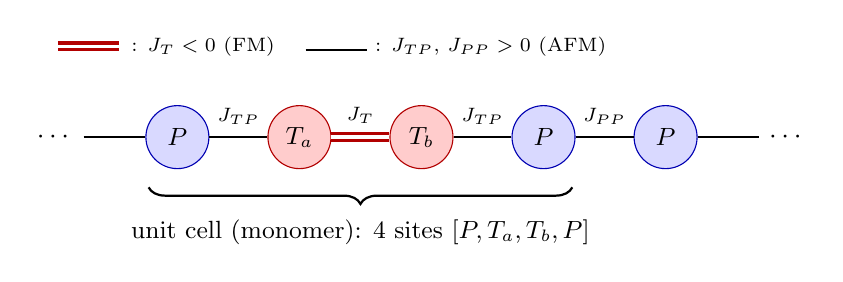
\begin{tikzpicture}[
    P/.style={circle,draw=blue!70!black,fill=blue!15,minimum size=8mm,inner sep=0pt,font=\small},
    T/.style={circle,draw=red!70!black,fill=red!20,minimum size=8mm,inner sep=0pt,font=\small},
    afm/.style={thick},
    fm/.style={very thick,red!70!black,double,double distance=1.2pt},
    jlab/.style={font=\scriptsize,midway,above=1pt},
    x=1.55cm
]

% left context
\node (l0) at (-1,0) {$\cdots$};

% unit cell : P - Ta - Tb - P
\node[P] (P1) at (0,0) {$P$};
\node[T] (Ta) at (1,0) {$T_a$};
\node[T] (Tb) at (2,0) {$T_b$};
\node[P] (P2) at (3,0) {$P$};

% next cell (context)
\node[P] (P3) at (4,0) {$P$};
\node (r0) at (5,0) {$\cdots$};

% intra-cell bonds
\draw[afm] (P1) -- (Ta) node[jlab]{$J_{TP}$};
\draw[fm]  (Ta) -- (Tb) node[jlab,black]{$J_{T}$};
\draw[afm] (Tb) -- (P2) node[jlab]{$J_{TP}$};

% context bonds and inter-cell bond
\draw[afm] (l0) -- (P1);
\draw[afm] (P2) -- (P3) node[jlab]{$J_{PP}$};
\draw[afm] (P3) -- (r0);

% brace for the unit cell
\draw[decorate,decoration={brace,amplitude=6pt,mirror},thick]
      ($(P1.south west)+(-0.05,-0.35)$) -- ($(P2.south east)+(0.05,-0.35)$)
      node[midway,below=8pt,font=\small]{unit cell (monomer): 4 sites $[P,T_a,T_b,P]$};

% legend
\node[font=\scriptsize,anchor=west] at (-1.1,1.15)
  {\tikz\draw[fm](0,0)--(0.5,0); : $J_T<0$ (FM)
   \quad
   \tikz\draw[afm](0,0)--(0.5,0); : $J_{TP},\,J_{PP}>0$ (AFM)};

\end{tikzpicture}
\end{center}

\noindent
The two red nodes $T_a,T_b$ tied by the double (ferromagnetic) $J_T$ bond
form the effective $S=1$ triangulene; the blue $P$ nodes are the
$S=\tfrac12$ phenalenyls. Translating the boxed unit cell $N$ times and
truncating at both ends produces the finite $4N$-site chain solved by ED.

\end{document}
